\section{Sentença}
\label{sec:sentence}
\index{Música!Sentença}
Uma sentença comumente tem oito compassos de comprimento e 
contém duas frases de quatro compassos \cite[pp. 48]{schoenberg1990fundamentos} \cite[pp. 21]{schoenberg1967fundamentals}.

\begin{itemize}
\item A primeira delas é chamada de frase de apresentação  e 
\item a segunda é a conclusão da sentença  \cite[pp. 58]{schoenberg1990fundamentos} \cite[pp. 58]{schoenberg1967fundamentals}.

\end{itemize}

Na frase de apresentação os primeiros dois compassos (ideia básica) são semelhantes aos dois últimos compassos,
de modo que pode existir uma simples repetição da ideia básica ou uma transposição;
também podem ser feitas pequenas mudanças na melodia ou harmonia sem que esta semelhança seja perdida \cite[pp. 48]{schoenberg1990fundamentos} \cite[pp. 21]{schoenberg1967fundamentals}.
Em muitos casos a ideia básica e a repetição complementar, tem uma relação de
forma \hyperref[sec:Tonica]{\textbf{tônica}} e forma dominante, 
respetivamente \cite[pp. 49]{schoenberg1990fundamentos} \cite[pp. 21]{schoenberg1967fundamentals}.

Dado que no inicio da sentença já incluímos uma repetição,
na conclusão da sentença serão feitas maiores variações;
o inicio da frase de conclusão é geralmente criado passando a frase de apresentação,
por um processo de extensão, expansão e logo redução, condensação e intensificação, 
neste processo 4 compassos são reduzidos a dois;
o final da frase de conclusão deve conter uma cadência adequada 
(cadência completa, semicadência, frígia, plagal, perfeita ou imperfeita),
em concordância com sua função na peça musical
\cite[pp. 59-59]{schoenberg1990fundamentos} \cite[pp. 58-59]{schoenberg1967fundamentals}.

A Figura \ref{fig:sentencestruct} mostra a estrutura de uma sentença. 
\begin{figure}[!h]
  \centering
    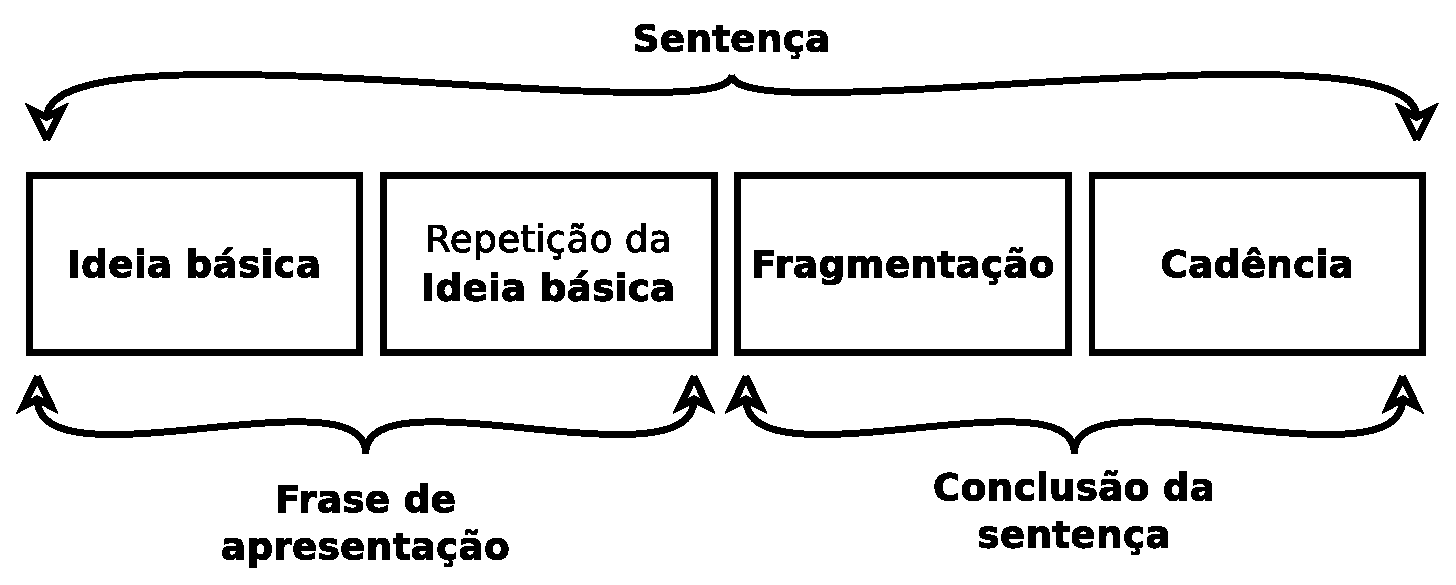
\includegraphics[width=\textwidth]{chapters/cap-musica-composer/sentencia.eps}
\caption{Estrutura de uma sentença.}
\label{fig:sentencestruct}
\end{figure}





Uma sentença tem uma forma mais trabalhada que o \hyperref[sec:Periodo]{\textbf{período}}, 
pois ela além de afirmar uma ideia como faz o período, a sentença desenvolve a ideia  
\cite[pp. 59]{schoenberg1990fundamentos} \cite[pp. 58]{schoenberg1967fundamentals}.

\begin{example}
Na Figura \ref{fig:sentence-ex1}, podemos ver uma sentença formada por 8 compassos;
os 2 primeiros compassos correspondem à ideia básica;
os seguintes 2 compassos tem uma repetição modificada da ideia básica, 
pois houve uma transposição em bloco e 
um diminuição especifica de um semitom nas notas com maior altura na ideia básica;
nos 4 últimos compassos da sentença é criada uma estrutura contrastante com a ideia básica terminando com uma cadência.
\end{example}

\begin{figure}[!h]
  \centering
    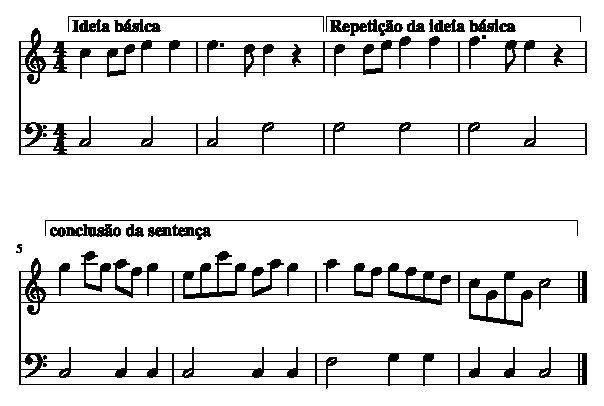
\includegraphics[width=\textwidth]{chapters/cap-musica-composer/sentence-ex1-1.eps}
\caption{Sentença de oito compassos.}
\label{fig:sentence-ex1}
\end{figure}
